\documentclass[11pt,a4paper]{article}
\usepackage{graphicx}
\usepackage[utf8]{inputenc}
\usepackage[T1]{fontenc}
\usepackage{blindtext}
\usepackage{enumitem}
\usepackage{hyperref}

\begin{document}
\tableofcontents
\listoffigures
\listoftables

\begin{flushleft}
\section{Informações Adicionais}

\subsection{Motivação}
Quando se pensa sobre os principais fatores que colaboram para o sucesso de
empresas a  satisfação do cliente no mercado de TI exerce um papel importante,
e \textit{user experience} é com certeza um dos principais fatores, os caminhos
para prover a \textit{user experience} são muitos, por exemplo prover qualidade
no serviço de usuário, pode ser um desses caminhos. Consequentemente vemos o
suporte ao usuário como sendo um serviço provido por uma empresa  ao seus
clientes com o objetivo de melhorar a experiência com o produto provido. Em
outras palavras o serviço de suporte ao usuário ajuda ao cliente resolver
qualquer problema que possa encontrar enquanto usa o produto ou serviço

\end{flushleft}

\subsubsection{Serviço de suporte ao usuário}
Primeiramente devemos definir o que é o serviço de suporte na área de TI,
podemos encontrar vários termos como:
\begin{itemize}[noitemsep]
  \item Suporte tecnico;
  \item Service Desk;
  \item Help Desk;
  \item Suporte ao Cliente;
  \item Suporte;
  \item Suporte ao usuário;
  \item Etc.
\end{itemize}

Basicamente esses termos definem a mesma coisa, mas cada um deles é focado
em diferentes aspectos do serviço, então para isso vamos focar no suporte
ao usuário, pois esse é mais comum e com isso evitamos ambiguidades.
Logo entende-se como suporte ao usuário um serviço provido por uma organização
para seus clientes para promover uma experiência com seu produto ou serviço,
resolvendo qualquer problema que o cliente possa encontrar enquanto usa o
serviço ou produto. Além disso não se  deve colocar qualquer restrição ao tipo
de problema que possa ser encontrado ou qualquer dúvida ou denuncia que o
cliente possa reportar.


\section{Execução do Projeto}
\begin{itemize}[noitemsep]
\item Fase 1 - Análise
	\begin{itemize}[noitemsep]
		\item Compreensão do contexto
		\item Formalizar os processos correntes (AS-IS)
		\item Analizar oas informações do sistema de log		
		\item Definir dos objetivos
		\item Definir os Fatores de Sucesso
		\item Identificar os envolvidos
		\item Análise das informações
	\end{itemize}		
\item Fase 2 - Otimização
	\begin{itemize}[noitemsep]
		\item Otimização dos processos identificados (TO-BE)	
		\item Documentação de novos processos	
	\end{itemize}
\item Fase 3 - Implantação
	\begin{itemize}[noitemsep]
		\item  Implantação dos novos processos
	\end{itemize}
\item Fase 4 - Validação
	\begin{itemize}[noitemsep]
		\item Implantação do processo de monitoramento	
	\end{itemize}

\end{itemize}

\section{Modelo AS-IS}
\subsection{Contexto}
	\paragraph{}
	O cenário usado como referência nesse trabalho é o de uma empresa que 
	fornece hardware e software para emissão de cupons fiscais emitidos no
	caixa. O produto de software é responsável por identificar o item quando passados no 
	identificador de código de barras. A solução de hardware é composta pelo identificador
	de código de barras, emissor de cupom fiscal e monitor.Como a empresa em questão é 
	provedora de dois items, o serviço de atendimento ao 
	usuário se faz necessário pois tais soluções podem apresentar algum defeito. O público alvo
	dessa empresa são supermercados ou quaisquer empreendimento que busca ter catalogados seus items
	e disponibiliza-los para venda.O contexto abordará somente o atendimento do usuário (supermercados) em 
	relação ao uso das duas soluções.
		
		O processo de suporte aos usuários das soluções se encontra disforme e não vem obtendo
	os resultatos esperados, causando insatisfação dos clientes, além de gastos por parte da empresa.
	Devido a esses problemas os usuários(supermercados) deixam de lucrar, agravando ainda mais a satisfação
	dos clientes. Buscando resolver esse problema e ainda agregar valor para o usuário utilizando provendo
	um serviço eficiente e eficaz. 
	Nos tópicos a seguir será mostrado os objetivos,fatores de sucesso, os processos
	identificados assim como uma analise do que foi encontrado 
	
	\paragraph{}A empresa solicitou que seu nome não fosse citado nos resultados aqui mostrados, esse pedido
	se fez necessário pois a mesma está sobre o processo de direito de imagem e venda.	
		
\subsection{Objetivos}
\begin{itemize}[noitemsep]
  \item Formalizar o processo atual
  \item Encontrar gargalos
  \item Otimizar processos
\end{itemize}

\subsection{Principais indicadores}
\begin{itemize}[noitemsep]
  \item Diminuição do tempo de processamento de uma requisição individual
  \item Diminuir a necessidade de tarefas humanas no processo de suporte
\end{itemize}

\subsection{Time do projeto}
\begin{itemize}[noitemsep]
  \item Operador de suporte
  \item Desenvolvedor Sênior
  \item Representante de Vendas
  \item Chefe de tecnologia
\end{itemize}




\subsection{Modelos dos processos}
\paragraph{}
Nessa seção vamos abordar a modelagem dos processos identificados no contexto,
os processos aqui mostrados usam a notação do BPMN para dar clareza e objetividade.
Proporcionando um padrão internacional de leitura dos mesmos.


\subsubsection{Gerência de requisição}
\begin{figure}[!h]
\caption{Gerencia de requisição}
\centering % para centralizarmos a figura
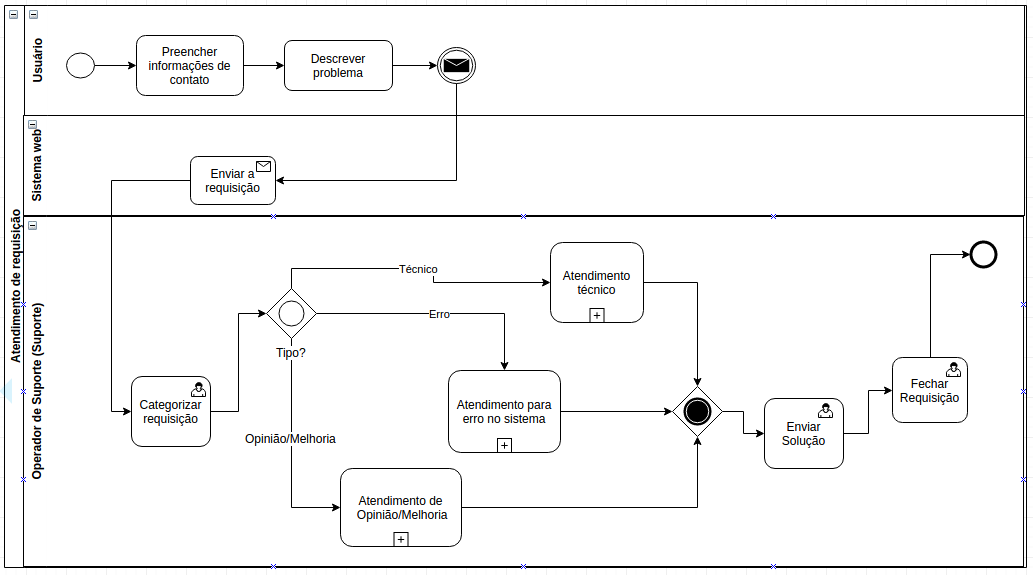
\includegraphics[width=15cm]{as-is/01_atendimento_de_requisicao.png}
\label{figura:atendimento_requisicao_as_is}
\end{figure}

\begin{itemize}[noitemsep]
	\item Preencher informações de contato
	\item Descrever problema
	\item Enviar requisição
	\item Enviar requisição
	\item Categorizar requisição
	\item Enviar Solicitação
	\item Fechar requisição
\end{itemize}

\subsubsection{Atendimento técnico}
asssss
\begin{figure}[!h]
\caption{Atendimento técnico}
\centering % para centralizarmos a figura
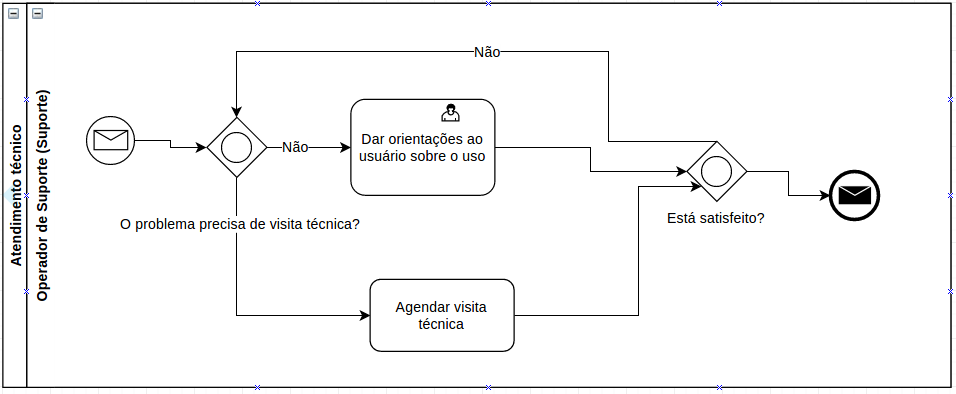
\includegraphics[width=15cm]{as-is/02_suporte_tecnico.png}
\label{figura:suporte_tecnico_as_is}
\end{figure}

\subsubsection{Atendimento para erro no sistema}

\begin{figure}[!h]
\caption{Atendimento para erro no sistema}
\centering % para centralizarmos a figura
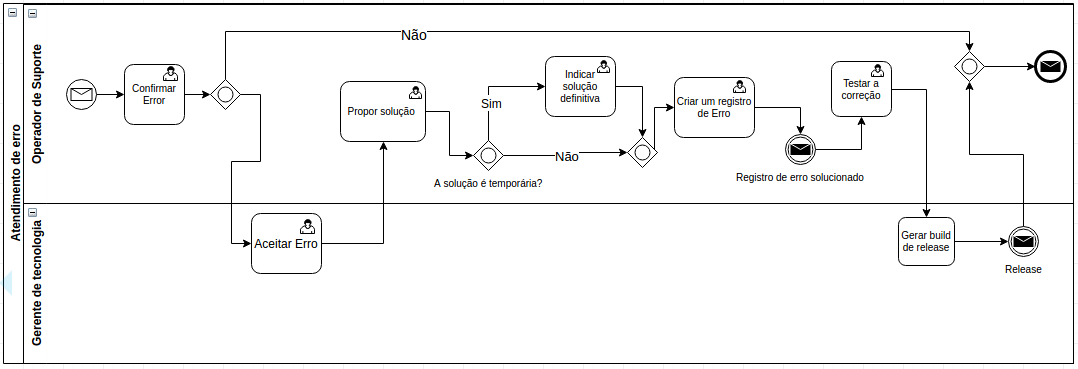
\includegraphics[width=16cm, height=5cm]{as-is/03_atendimento_de_erro.png}
\label{figura:atendimento_de_erro_as_is}
\end{figure}
\begin{itemize}
	\item Confirmar erro
	\item Aceitar Erro
	\item Propor Solução
	\item Indicar Solução definitiva
	\item Criar registro
\end{itemize}




\subsubsection{Atendimento de Opinião/Melhoria}
fffffffffff
\begin{figure}[!h]
\caption{Atendimento de Opinião/Melhoria}
\centering % para centralizarmos a figura
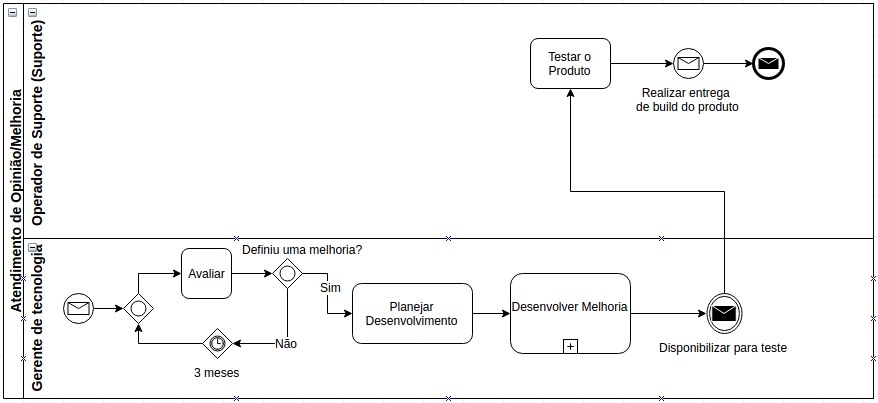
\includegraphics[width=15cm]{as-is/04_atendimento_de_melhoria.png}
\label{figura:atendimento_de_melhoria_as_is}
\end{figure}


\subsection{Conclusão e análise}
\begin{itemize}[noitemsep]
  \item Processos indefinidos
  \item Ausencia de monitoramentos
  \item Ausencia de uma base de conhecimento
  \item Ausencia de autenticação de usuário
  \item Processos de longo tempo de execução
  \item Reporte insuficiênte para o cliente
\end{itemize}

\section{Padrões e Normas}
\subsection{ITIL}
A ITIL define serviço como um meio intangível de entregar valor aos clientes,
facilitando resultados sem ter que assumir custos e riscos extras.

E a ITIL mapeia todo o ciclo de vida dos serviços através de 5 pilares:
\begin{itemize}[noitemsep]
  \item Estratégia do Serviço
  \item Desenho de Serviço
  \item Transição de Serviço
  \item Operação do Serviço
  \item Melhoria Continuada
\end{itemize}

Estratégia do Serviço (“Service Strategy”): É aqui que são tomadas as deciões estratégicas relacionadas aos serviços que vão ser desenvolvidos. Serviços que ajudam na identificação de requisitos e outras necessidades que ajudam a alcançar os objetivos do negócio.

Desenho de Serviço (“Service Design”): Basicamente desenha o que a estratégia decidiu, tendo em mente os fatores de utilidade e garantia, tomando por base as características esperadas para os serviços e culminando na elaboração e descrição de especificações dos serviços.

Transição de Serviço (“Service Transition”): Tem por foco o gerenciamento de mudanças, prevendo para tal fim a condução de ações voltadas à implantação de serviços. Move os serviços para o ambiente de produção. Os serviços são desenvolvidos, testados e liberados de forma controlada.

Operação do Serviço (“Service Operation”): Aqui estão os processos do dia-a-dia, que mantém os serviços funcionando assegurando que seus objetivos sejam alcançados, baseando-se para isto, em acordos de níveis de serviços (SLAs, sigla do inglês “Service-level Agreements”).

Melhoria Contínua do Serviço (“Continual Service Improvement”): Busca constante pela evolução dos serviços, aplicando para isto conceitos oriundos de técnicas como o ciclo PDCA (sigla do inglês “Plan-Do-Check-Act”).

Esses pilares, se destrinchados, nos fornecem um total de 26 processos e 4 funções, aprofundando o conceito de como estruturar um serviço de acordo com áreas, fases do ciclo de vida e funções.



As práticas de ITIL procuram fornecer o suporte necessário para que tais serviços estejam em sintonia com as necessidades do negócio.Dentre os benefícios que podem ser obtidos a parte da utilização das técnicas que compõem ITIL, pode-se destacar:


\begin{itemize}[noitemsep]
	\item Melhorias na satisfação dos clientes/áreas dependentes de um ou mais serviços;
	\item Maior eficiência operacional;
	\item Redução nos custos e nos esforços desprendidos pela área de TI cumprimento de uma ampla gama de atividades;
\end{itemize}



\section{ Melhoria de processo (TO - BE)}

\begin{itemize}[noitemsep]
	\item Gestão de Conhecimento e Auto-Ajuda
	\item	Para base de conhecimento, será preciso incluir
	\begin{itemize}[noitemsep]
		\item Manual para suporte dos usuários
		\item Documentação completa dos produtos de software
		\item Documentação de Problemas comuns
		\item Base de dados de erros e suas workarounds
		\item Base de dados de improvement sugestions
	\end{itemize}
	A base de conhecimento será lançada como uma extensão do
	suporte web page
	\item Monitoramento de performace
\end{itemize}


Como primeira ação foi necessário achar os indicadores chave de performace,
onde foi possivel mapear o relacionamento desses indicadores chave com os fatores
criticos de sucesso

















\section{Referências}
Alison Cartlidge, A. H. (2007). An Introductory Overview of ITIL v3. The UK Chapter of the itSMF.\\
Itil V3 Library - ITSMF \\

\end{document}
